\rhead{实验与结果分析}
\chapter{实验与结果分析}

%@@@@@@@@@@@@@@@@@@@@@@@@@@@@
\section{数据集及预处理}
实验所用的所有数据均来自IsoBase数据库\cite{park2011isobase}。Isobase数据库是被普遍使用的生物PPI网络数据库,因此我们选择了这个数据集。该数据集包含了四种生物的PPI网络数据,分别是Saccharomyces cerevisiae(简写为S.cerevisiae或sc),Drosophila melanogaster(简写为D.melanogaster或dm),Caenorhabditis elegans(简写为C.elegans或ce)以及Homo sapiens(简写为H.sapiens或hs)。本文使用\cite{zhang2016method}的方法,构造了四个对应的动态PPI网络,并且实验所用的静态PPI网络是从对应的动态PPI网络中抽取的分时网络,而不是原PPI网络。对于抽取的分时网络,每种生物的网络详细信息见表\ref{table:1.1}。

\begin{table}[htbp]
    \centering
    \caption{实验所用的静态PPI网络(分时网络)}
    \label{table:1.1}
    \begin{tabular}{cccc}
         \hline 物种&点数&边数&平均点度\\
         \hline C.elegans&2974&2653&1.78\\
         D.melanogaster&7387&14004&3.79\\
         H.sapiens&10296&30349&5.90\\
         S.cerevisiae&5523&46207&16.73\\
         \hline
    \end{tabular}
\end{table}

而四个动态PPI网络的详细信息,见表\ref{table:1.2}。

\begin{table}[htbp]
    \centering
    \caption{实验所用的动态PPI网络}
    \label{table:1.2}
    \begin{tabular}{cccc}
         \hline 物种&T&点数&平均边数\\
         \hline C.elegans&15&2974&1896.87\\
         D.melanogaster&15&7387&9995.27\\
         H.sapiens&15&10296&21772.73\\
         S.cerevisiae&15&5523&32990.53\\
         \hline
    \end{tabular}
\end{table}

%@@@@@@@@@@@@@@@@@@@@@@@@@@@@@@@@@
\section{实验方法与环境}
本文使用了全局比对算法中的四种经典算法作为和本文算法的对比,分别是IsoRank\cite{singh2008global},SPINAL\cite{aladaug2013spinal},L-GRAAL\cite{malod2015graal}和PROPER\cite{kazemi2016proper}算法。SGOPT算法全部代码由Java构成,并且运行在Linux Ubuntu环境下,详细的环境参数见表\ref{table:2}。

对于这四种不同的静态比对算法,首先使用方案一和方案二产生两种不同的比对结果,其次,本文采用SGOPT在方案一产生的比对结果上进行优化,产生第三种比对结果,对比这三种情况下的比对结果的好坏程度。至于如何衡量比对结果的好坏,本文首先以CE指标和运行时间作为主要考量的指标,然后再比较本文中新定义的四个动态比对衡量指标,即DEC,DICS,DS$^3$和DTWC。

\begin{table}[htbp]
    \centering
    \caption{实验运行环境}
    \label{table:2}
    \begin{tabular}{l|l}
         \hline 
         CPU&Intel Core i7-4790K, 4.00GHz\\
         \hline
         内存&16G\\
         \hline
         操作系统&Linux Ubuntu 14.04LTS,64位\\
         \hline
    \end{tabular}
\end{table}

本文使用\textit{算法-方案一}和\textit{算法-方案二}来表示某种算法其在方案一下和方案二下产生的比对结果,而\textit{SGOPT-算法}表示某种算法在方案一下产生的结果经过SGOPT优化后得到的第三种比对结果。例如,\textit{IsoRank-方案一}就表示IsoRank算法在方案一下产生的比对结果,\textit{SGOPT-IsoRank}就表示SGOPT优化这个结果产生的新的比对结果。

为了简单起见,本文用\textit{生物1-生物2}来表示对\textit{生物1}的静态PPI网络与\textit{生物2}的动态PPI网络进行比对所得到的比对结果。例如\textit{ce-dm}表示将生物\textit{C.elegans}和\textit{D.melanogaster}进行比对得到的结果。

除了对比SGOPT与其他的静态比对算法,本文还测试了SGOPT算法的两个参数对SGOPT效果的影响。

%@@@@@@@@@@@@@@@@@@@@@@@@@@@@@@@@@@@@@
\section{$\alpha,\beta$参数对结果的影响}

\subsection{$\beta$参数的影响}
参数$\beta$影响的是每次删掉的匹配点对数,因此$\beta$越大,删掉的匹配点对数便越多,二分图便越大,导致一次迭代的时间就越长。图\ref{beta}是不同$\beta$情况下SGOPT算法的运行结果。从图\ref{beta1}中可以看到,对于一个固定的$\beta$,运行时间越长,则比对的效果越好。另一方面,在同样的运行时间下,越小的$\beta$有越好的效果,$\beta=600$时,SGOPT甚至不能提高初始比对结果的CE指标,这是因为当一轮迭代中删去的匹配点对过多的时候,SGOPT面对的是一个需要全局优化的局面,而SGOPT只适于局部优化的情况,所以在全局优化的情况下,SGOPT并不能很快找到一个拥有更高CE指标的比对结果。所以SGOPT适合$\beta$比较小的情况。

而图\ref{beta2}则是$\beta$比较小的时候,SGOPT算法的实验结果。可以看到此时,不同$\beta$下的结果并没有明显的差别。最终,本文设置$\beta=35$做为实验的默认参数。

\begin{figure}[htbp]
    \subfigure[$\beta$从50到2000变化时(步长50)的实验结果]{
        \begin{minipage}[b]{0.5\linewidth}
            \centering
            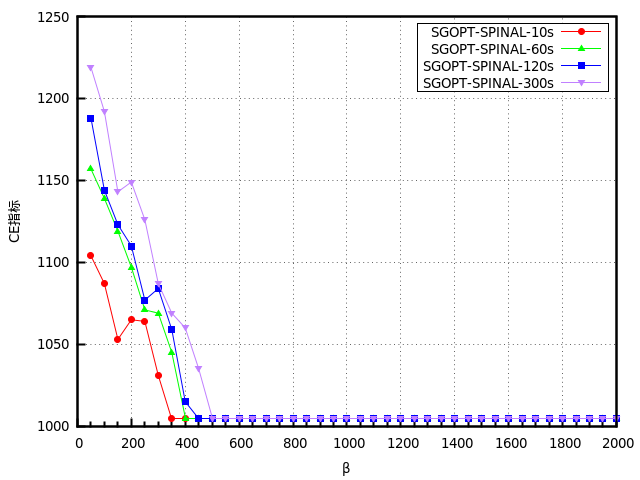
\includegraphics[width=\linewidth]{pic/beta1.png}
            \label{beta1}
        \end{minipage}
    }
   \subfigure[$\beta$从5到50变化时(步长3)的实验结果]{
        \begin{minipage}[b]{0.5\linewidth}
            \centering
            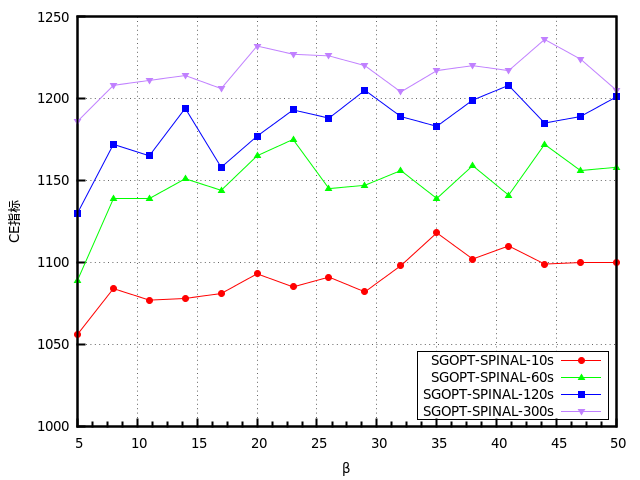
\includegraphics[width=\linewidth]{pic/beta2.png}
            \label{beta2}
        \end{minipage}
    }
    \caption{在\textit{ce-dm}实验组下,不同$\beta$值对\textit{SGOPT-SPINAL}的实验结果的影响。不同曲线代表不同的运行时间。 }
    \label{beta}
\end{figure}

%@@@@@@@@@@@@@@@@@@@@@@@@@@@@@@@@@@@@@@@@@@@@@@@@@@
\subsection{$\alpha$参数的影响}

$\alpha$参数控制SGOPT算法的迭代轮数,从SGOPT算法可以看出,随着迭代论次的不断变化,比对的CE指标会不断得到提高,可以从图\ref{alpha}中看出来。为了进一步考察迭代轮数对算法结果的影响,参见图\ref{alphad},从中可以看出,随着迭代轮次的加多,CE指标得到提高的机会越来越少,说明算法有个收敛的过程,虽然理论上,随着迭代次数的增加,CE指标会越来越高,但是考虑到运行时间的关系,本文最终设置$\alpha=15000$作为实验的默认参数。

\begin{figure}[htbp]
    \subfigure[CE指标随迭代论次变化的结果]{
        \begin{minipage}[b]{0.5\linewidth}
            \centering
            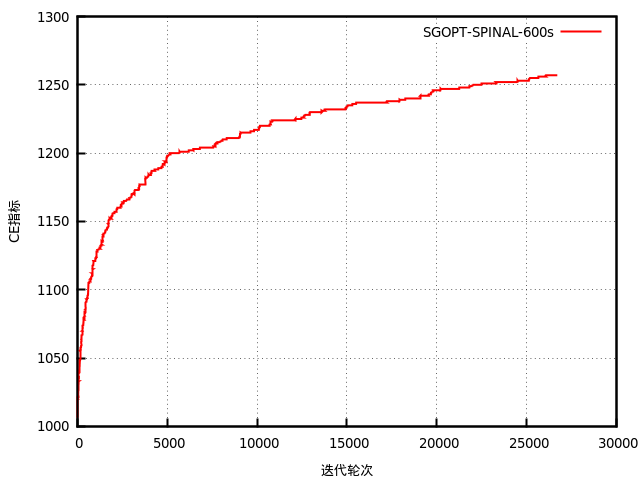
\includegraphics[width=\linewidth]{pic/alpha.png}
            \label{alpha}
        \end{minipage}
    }
   \subfigure[CE指标(差值)随迭代论次变化的结果]{
        \begin{minipage}[b]{0.5\linewidth}
            \centering
            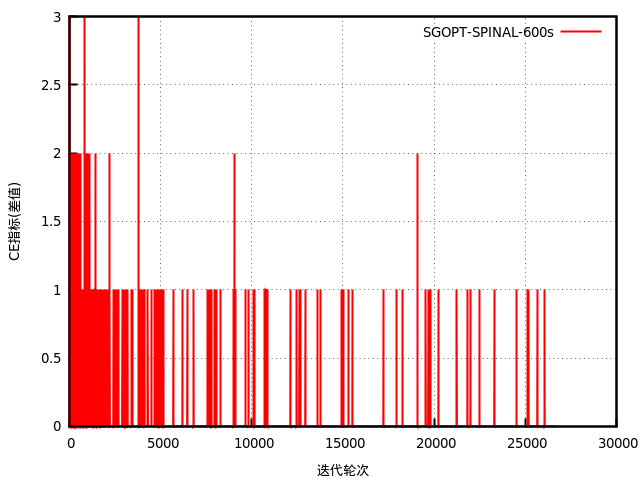
\includegraphics[width=\linewidth]{pic/alphad.png}
            \label{alphad}
        \end{minipage}
    }
    \caption{在\textit{ce-dm}实验组下,\textit{SGOPT-SPINAL}的CE指标随迭代论次增加而变化的实验结果。}
    \label{alphaall}
\end{figure}


%@@@@@@@@@@@@@@@@@@@@@@@@@@@@@@@@@@@@@@@@@
\section{不同算法之间的比较}

对于实验中要比较的四种静态算法,本文使用它们的默认参数,见表\ref{table:3}。

\begin{table}[htbp]
    \centering
    \caption{静态比对算法与运行参数}
    \label{table:3}
    \begin{tabular}{ccc}
         \hline 算法&命令行&参数\\
         \hline IsoRank&-alpha $\alpha$ -I 50&$\alpha=1$\\
         SPINAL&-II -alpha $\alpha$&$\alpha=1$\\
         L-GRAAL&-alpha $\alpha$&$\alpha=1$\\
         PROPER&$-l$ $l$ $-r$ $r$&$l=500,r=1$\\
         \hline
    \end{tabular}
\end{table}

%@@@@@@@@@@@@@@@@@@@@@@@@@@@@@@@@@@@@
\subsection{CE指标与运行时间}
图\ref{ce-dm}是\textit{ce-dm}实验组的结果。图\ref{ce-dm-CE}是CE指标的实验结果,图\ref{ce-dm-Time}则是运行时间的结果。从CE指标来看,SGOPT算法好于方案一,差于方案二,唯一的例外是对于IsoRank这个算法,SGOPT的优化效果远远超出了预期。从运行时间上来看,SGOPT的运行时间与方案一相比,只多了其调整比对所运行的时间。对于方案二,由于需要对静态网络和每个分时网络逐一进行比对,整个过程十分耗时。综合考虑,SGOPT在效果上比方案一好,在时间上远快于方案二,不失为一种折中的方案。

\begin{figure}[htbp]
    \subfigure[CE指标]{
        \begin{minipage}[b]{0.5\linewidth}
            \centering
            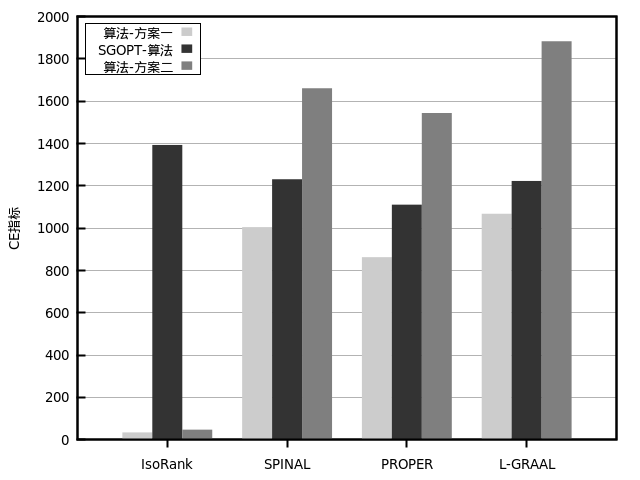
\includegraphics[width=\linewidth]{pic/ce-dm-CE.png}
            \label{ce-dm-CE}
        \end{minipage}
    }
   \subfigure[运行时间]{
        \begin{minipage}[b]{0.5\linewidth}
            \centering
            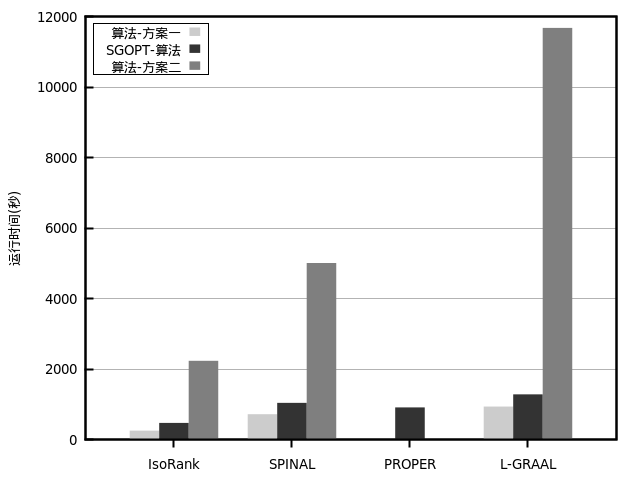
\includegraphics[width=\linewidth]{pic/ce-dm-Time.png}
            \label{ce-dm-Time}
        \end{minipage}
    }
    \caption{在\textit{ce-dm}实验组下,四种静态算法在三种方案下的实验结果。}
    \label{ce-dm}
\end{figure}

对于剩下的实验组,结果可见图\ref{ce-hs},\ref{ce-sc},\ref{dm-hs},\ref{dm-sc},\ref{hs-sc}。可以看到结果是类似的。在\textit{hs-sc}实验组中,SGOPT对SPINAL的优化效果,甚至好于SPINAL在方案二下的结果。

值得一提的是PROPER算法,从实验中可以看到PROPER算法无论从时间上还是CE指标上,都是好于SGOPT的。但是值得注意的是在本实验中$T=15$,对于SGOPT算法来说很难凸显它的优势,因为实际情况中的动态PPI网络都是时间跨度比较小的网络。但是本文的算法同样适用于除PPI网络比对之外的其他的网络比对问题,在T较大的情况下,SGOPT算法的时间优势才得以体现。

\begin{figure}[htbp]
    \subfigure[CE指标]{
        \begin{minipage}[b]{0.5\linewidth}
            \centering
            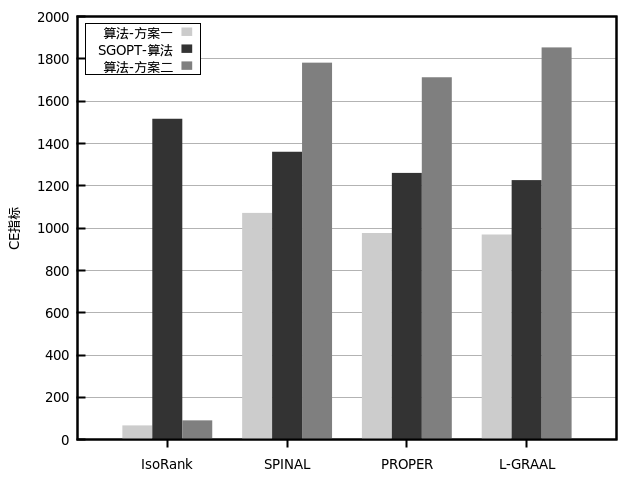
\includegraphics[width=\linewidth]{pic/ce-hs-CE.png}
            \label{ce-hs-CE}
        \end{minipage}
    }
   \subfigure[运行时间]{
        \begin{minipage}[b]{0.5\linewidth}
            \centering
            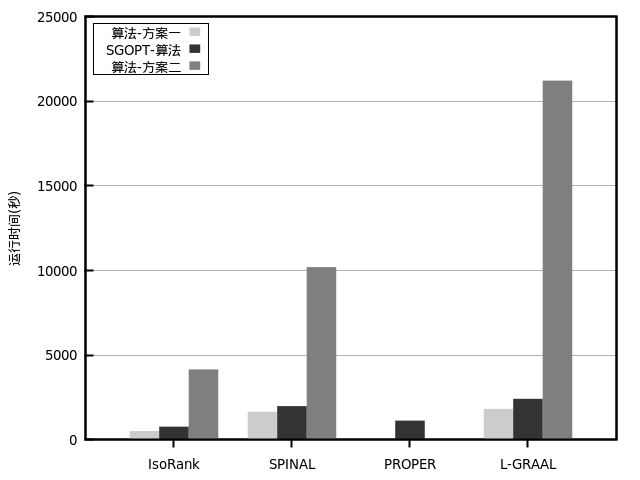
\includegraphics[width=\linewidth]{pic/ce-hs-Time.png}
            \label{ce-hs-Time}
        \end{minipage}
    }
    \caption{在\textit{ce-hs}实验组下,四种静态算法在三种方案下的实验结果。}
    \label{ce-hs}
\end{figure}


\begin{figure}[htbp]
    \subfigure[CE指标]{
        \begin{minipage}[b]{0.5\linewidth}
            \centering
            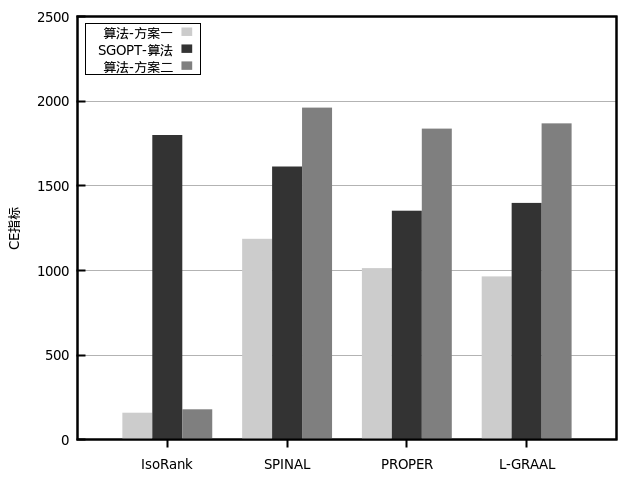
\includegraphics[width=\linewidth]{pic/ce-sc-CE.png}
            \label{ce-sc-CE}
        \end{minipage}
    }
   \subfigure[运行时间]{
        \begin{minipage}[b]{0.5\linewidth}
            \centering
            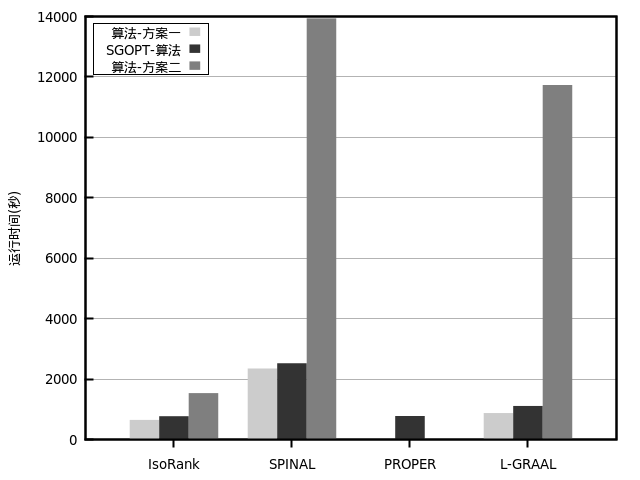
\includegraphics[width=\linewidth]{pic/ce-sc-Time.png}
            \label{ce-sc-Time}
        \end{minipage}
    }
    \caption{在\textit{ce-sc}实验组下,四种静态算法在三种方案下的实验结果。}
    \label{ce-sc}
\end{figure}

\begin{figure}[htbp]
    \subfigure[CE指标]{
        \begin{minipage}[b]{0.5\linewidth}
            \centering
            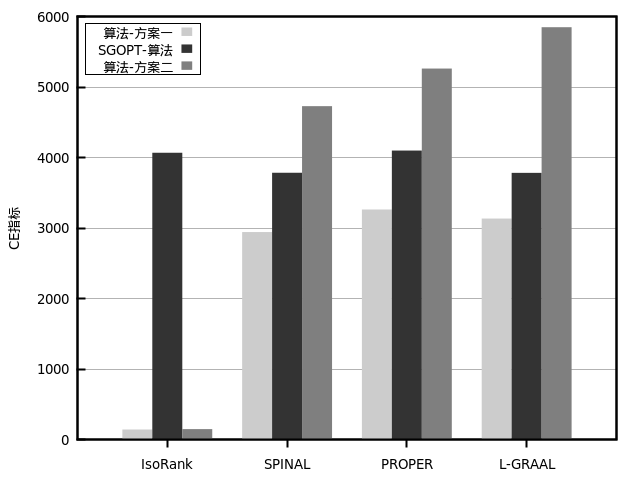
\includegraphics[width=\linewidth]{pic/dm-hs-CE.png}
            \label{dm-hs-CE}
        \end{minipage}
    }
   \subfigure[运行时间]{
        \begin{minipage}[b]{0.5\linewidth}
            \centering
            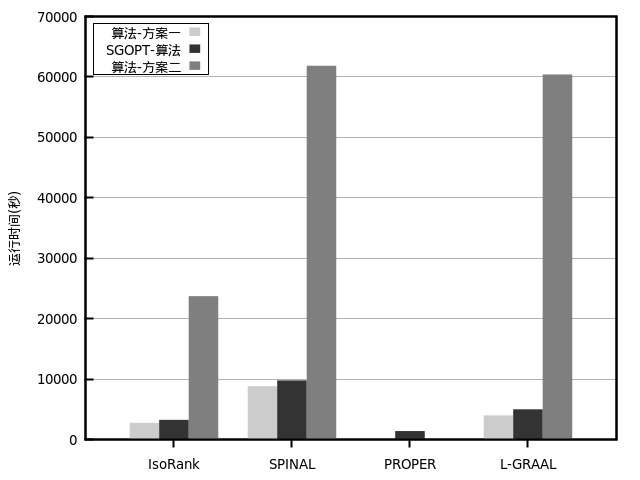
\includegraphics[width=\linewidth]{pic/dm-hs-Time.png}
            \label{dm-hs-Time}
        \end{minipage}
    }
    \caption{在\textit{dm-hs}实验组下,四种静态算法在三种方案下的实验结果。}
    \label{dm-hs}
\end{figure}

\begin{figure}[htbp]
    \subfigure[CE指标]{
        \begin{minipage}[b]{0.5\linewidth}
            \centering
            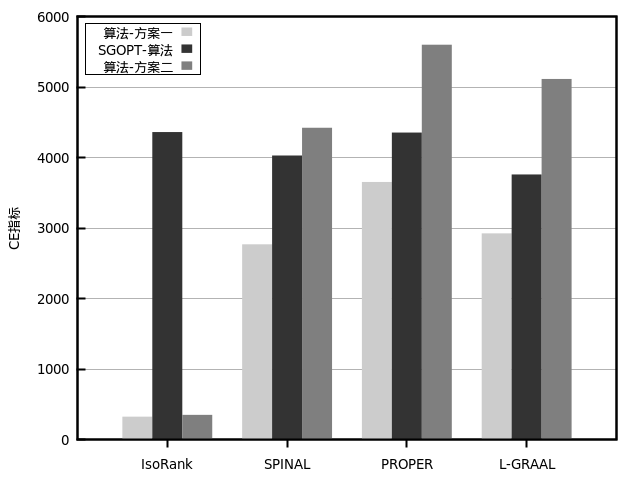
\includegraphics[width=\linewidth]{pic/dm-sc-CE.png}
            \label{dm-sc-CE}
        \end{minipage}
    }
   \subfigure[运行时间]{
        \begin{minipage}[b]{0.5\linewidth}
            \centering
            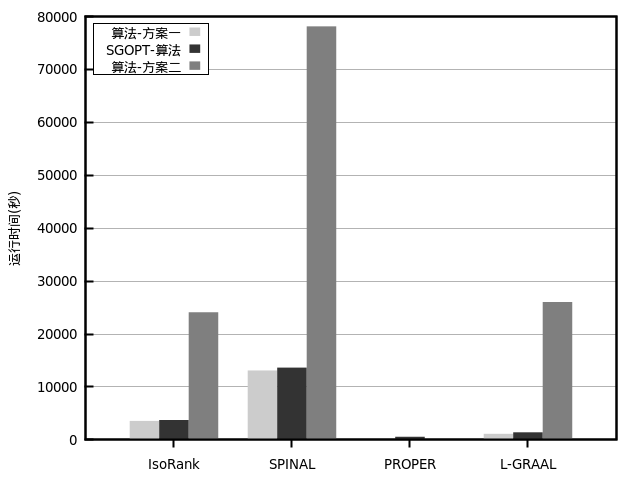
\includegraphics[width=\linewidth]{pic/dm-sc-Time.png}
            \label{dm-sc-Time}
        \end{minipage}
    }
    \caption{在\textit{dm-sc}实验组下,四种静态算法在三种方案下的实验结果。}
    \label{dm-sc}
\end{figure}

\begin{figure}[htbp]
    \subfigure[CE指标]{
        \begin{minipage}[b]{0.5\linewidth}
            \centering
            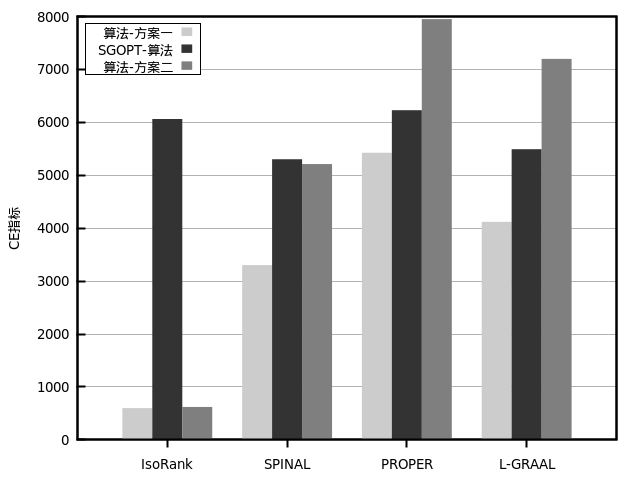
\includegraphics[width=\linewidth]{pic/hs-sc-CE.png}
            \label{hs-sc-CE}
        \end{minipage}
    }
   \subfigure[运行时间]{
        \begin{minipage}[b]{0.5\linewidth}
            \centering
            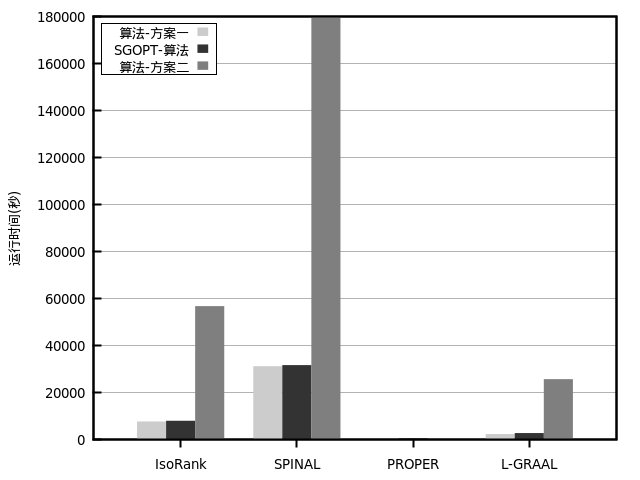
\includegraphics[width=\linewidth]{pic/hs-sc-Time.png}
            \label{hs-sc-Time}
        \end{minipage}
    }
    \caption{在\textit{hs-sc}实验组下,四种静态算法在三种方案下的实验结果。}
    \label{hs-sc}
\end{figure}

\subsection{CE指标的提高程度}
SGOPT算法对于四种比对算法在不同实验组下,对CE指标的优化的结果见图\ref{improveCE}。可以看到SGOPT对IsoRank的优化超出了预期,对于其他三种算法,SGOPT能够优化20\%到60\%。可见SGOPT是一种行而有效的优化框架。
\begin{figure}[!htbp]
    \centering
    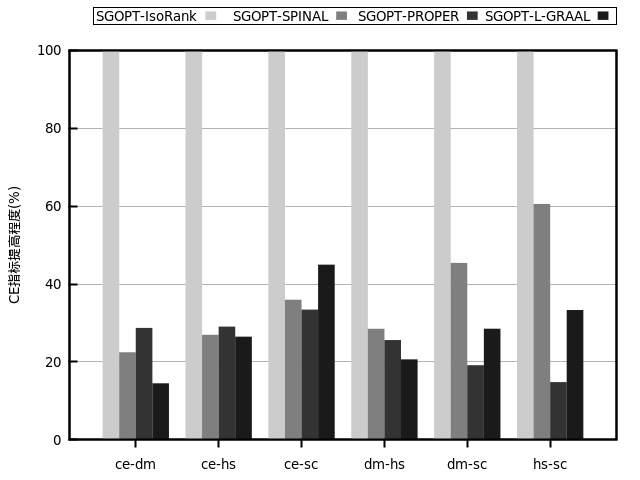
\includegraphics[width=0.8\linewidth]{pic/improveCE.png}
    \caption{在不同实验组下,SGOPT对于四种比对算法的CE指标的提高程度}
    \label{improveCE}
\end{figure}

%@@@@@@@@@@@@@@@@@@@@@@@@@@@@@@@@@@@@@2
\section{DEC,DICS,$DS^3$,DTWEC指标的对比}
目前为止所有的实验采用的衡量指标都是CE指标,那么在另外的指标下,SGOPT算法的效果又如何呢?图\ref{improveOther}是SGOPT算法对于其他指标的优化效果。

从不同的比对算法来看,对于IsoRank和SPINAL,可以看到SGOPT在所有实验组下都能对四项指标进行一定程度的优化。对于IsoRank,优化程度是超出预期的好,对于SPINAL,优化程度从20\%到60\%不等。在实验组\textit{hs-sc}中,对SPINAL的优化效果最好。而对于PROPER和L-GRAAL算法,SGOPT的优化效果则不如前两者。并且,SGOPT对于DICS和DS$^3$指标在实验组\textit{ce-dm,ce-hs,ce-hs,dm-hs}下没有任何优化效果。

从不同的衡量指标来看,DEC指标的优化效果最好,接下来的则是DTWEC指标,剩下的两个指标的优化程度则较差。

从不同实验组来看,可以发现在实验组\textit{dm-hs,dm-sc,hs-sc}下,SGOPT的优化效果教其他实验组好,猜想这是因为SGOPT的目标是最大化保留边的数目,而这一指标在两个网络都拥有很多边的情况下,会有更好的优化空间,所以结果也会较好。

\begin{figure}[!t]
    \subfigure[DEC指标提高程度]{
        \begin{minipage}[b]{0.5\linewidth}
            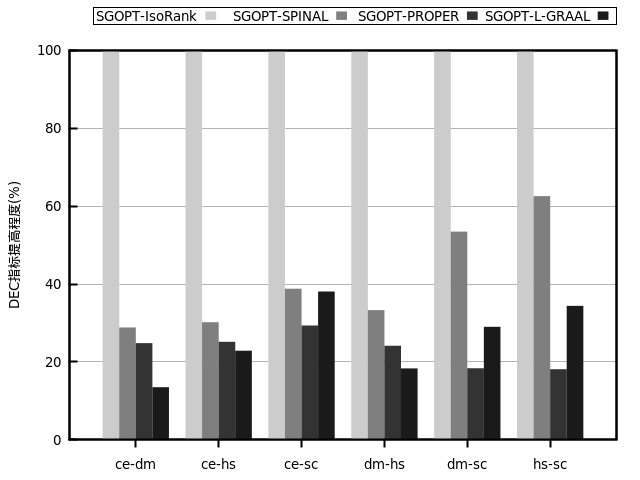
\includegraphics[width=\linewidth]{pic/improveDEC.png}
            \label{improveDEC}
        \end{minipage}
    }
   \subfigure[DICS指标提高程度]{
        \begin{minipage}[b]{0.5\linewidth}
            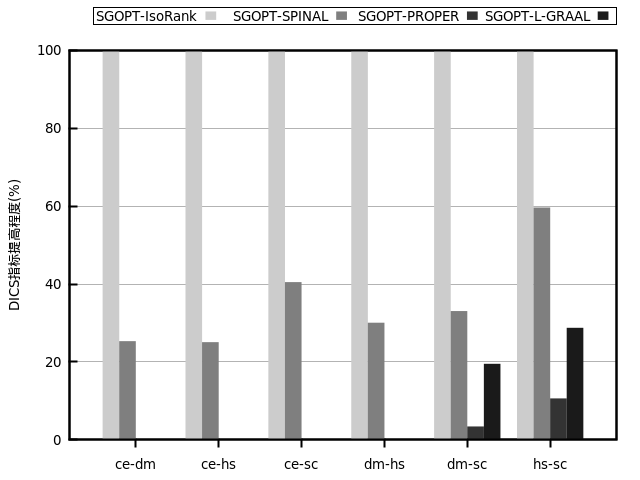
\includegraphics[width=\linewidth]{pic/improveDICS.png}
            \label{improveDICS}
        \end{minipage}
    }
     \subfigure[DS$^3$指标提高程度]{
        \begin{minipage}[b]{0.5\linewidth}
            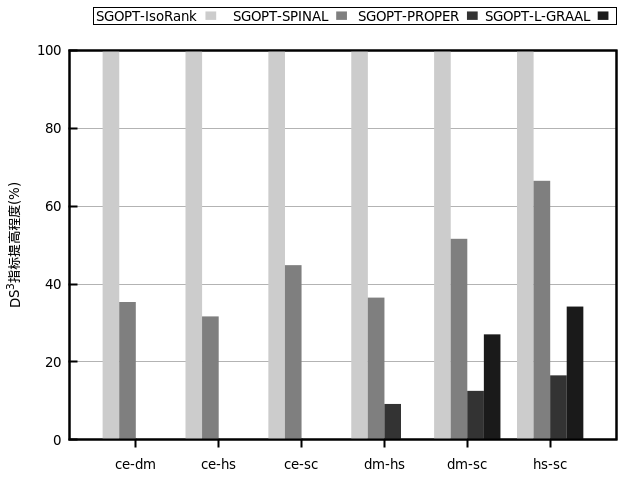
\includegraphics[width=\linewidth]{pic/improveDS3.png}
            \label{improveDS3}
        \end{minipage}
    }
     \subfigure[DTWEC指标提高程度]{
        \begin{minipage}[b]{0.5\linewidth}
            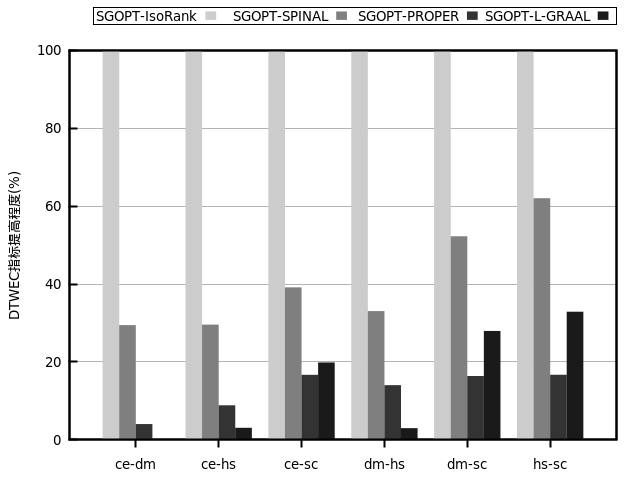
\includegraphics[width=\linewidth]{pic/improveDTWEC.png}
            \label{improveDTWEC}
        \end{minipage}
    }
    \caption{SGOPT算法对于其他四项指标的优化效果}
    \label{improveOther}
\end{figure}


